\section{Results}
\label{sec:results}

\subsection{Exploratory Sweeps}

\emph{Untuned baselines favor early triggering (\cref{fig:dose}).}  Against an
uncertainty-blind arrival-gap rule and an unpadded current-margin rule, the
predictive rule with $T_h=2.0$\,s appears strong.  With rate-limited recovery
($a_{\max}=1.0$), the uncertainty-blind rule fails first as severity grows, the
unpadded rule collides in many moderate- and high-severity episodes, and the
predictive rule records no collision on this exploratory seed grid.  Earlier
action can therefore matter in the simulator, but this does not show that
prediction is needed, because a padded current-margin rule can also act early.

\begin{figure}[!t]
  \centering
  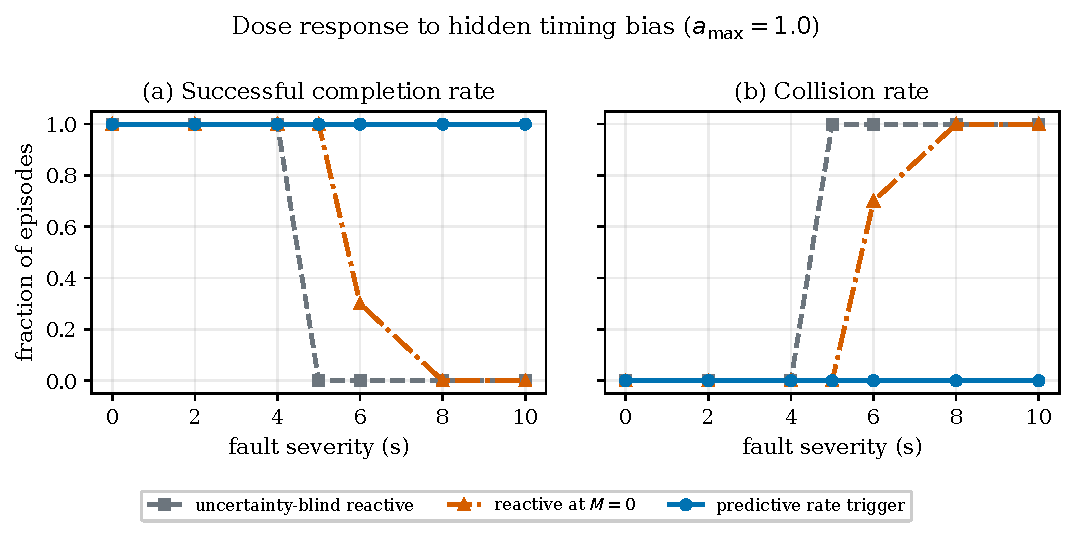
\includegraphics[width=\columnwidth]{fig_dose.pdf}
  \caption{Exploratory single-margin dose response with $T_h=2.0$\,s and
  $a_{\max}=1.0$: (a) successful completion rate and (b) collision rate over 40
  paired noise seeds per severity.  \Cref{fig:boundary} adds an in-sample
  fixed-pad comparator.}
  \label{fig:dose}
\end{figure}

\emph{The observed boundary is narrow (\cref{fig:boundary}).}  The plotted
difference is the mean elapsed time of the selected fixed pad minus that of the
predictive rule, so positive values favor prediction, and the fixed pad is
selected in-sample at every setting.  Under the slowest recovery
($a_{\max}=0.5$), the predictive rule finishes about $0.56$\,s sooner; the sign
changes as recovery becomes faster, reaching $-1.31$\,s at $a_{\max}=3.0$.  In
the degradation-shape sweep, the predictive rule records collisions at $p=0.3$
and $p=0.5$, where no tested fixed pad succeeds in every episode either; it is
about $1.23$\,s faster at $p=0.7$ and slower than the selected fixed pad from
$p=0.9$ onward.  These differences are small relative to episodes of roughly
25--30\,s, and the in-sample selection supports no inferential claim.

\begin{figure}[!t]
  \centering
  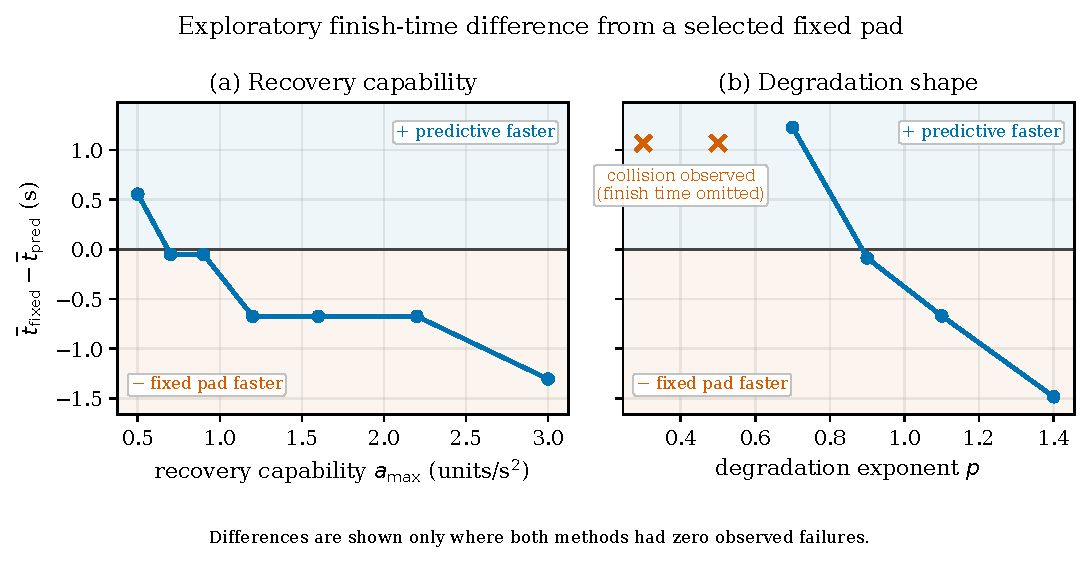
\includegraphics[width=\columnwidth]{fig_boundary.pdf}
  \caption{Exploratory elapsed-time difference between the selected fixed pad
  and the $T_h=2.0$\,s predictive rule across (a) recovery capability and (b)
  degradation shape at $a_{\max}=0.8$.  Positive values favor prediction.
  Differences are shown only where both rules recorded no failure; crosses mark
  settings in which the predictive rule collides and no tested fixed pad
  succeeds in every episode.}
  \label{fig:boundary}
\end{figure}

\subsection{Seed-Disjoint Single-Margin Evaluation}

The equal-budget searches select $\rho=2.5$\,s and $T_h=2.5$\,s
(\cref{tab:single-margin}).  On the 6,750 held-out conflict episodes, the fixed
rule succeeds in all episodes and records no collision.  The tuned predictive
rule succeeds in 6,748 and records two collisions, one at each of the two highest
severities with $a_{\max}=0.5$ and $p=0.7$.  Its successful-only mean elapsed
time is $26.577$\,s, compared with $27.690$\,s for the fixed rule, but these
means condition on different success sets.  We therefore attach no paired
interval and claim no efficiency advantage.  For context, the retained
$T_h=2.0$\,s rule records 172 collisions on the same held-out set.

\begin{table}[!t]
  \centering
  \caption{Seed-Disjoint Single-Margin Test Results over 6,750 Conflict
  Episodes per Arm}
  \label{tab:single-margin}
  \footnotesize
  \setlength{\tabcolsep}{3.5pt}
  \begin{tabular}{@{}llrrr@{}}
    \toprule
    Rule & Parameter & Collisions & Successes & Mean time (s) \\
    \midrule
    Fixed pad, tuned & $\rho=2.5$\,s & 0 & 6,750 & 27.690 \\
    Predictive, tuned & $T_h=2.5$\,s & 2 & 6,748 & 26.577 \\
    Predictive, retained & $T_h=2.0$\,s & 172 & 6,578 & 25.990 \\
    \bottomrule
  \end{tabular}

  \vspace{3pt}
  \parbox{\columnwidth}{\scriptsize Mean elapsed time is averaged over
  successful episodes only and therefore conditions on different success sets
  for different rules.}
\end{table}


In the 2,250 held-out clear episodes, both tuned rules complete without
collision.  The fixed rule yields unnecessarily in $1800/2250$ episodes
(80.0\%), and the predictive rule in $1358/2250$ (60.4\%).  This is evidence of
fewer interventions on the specified clear grid, not a safety-adjusted
performance gain.  The largest upper endpoint of the pointwise 95\% Wilson
collision intervals is $0.025$ for the fixed rule and $0.037$ for the
predictive rule.

\subsection{Seed-Disjoint Coordination Evaluation}

The redesigned geometry first passes a falsification check: without
intervention, all 1,620 held-out conflict runs reach the exit but contain both a
zone-occupancy collision and a headway violation, so none succeeds
(\cref{tab:coordination}).  These runs consume no measurement noise and are
therefore deterministic repeats within each physical scenario; their count
verifies coverage of the grid, not 1,620 independent safety trials.

\begin{table}[!t]
  \centering
  \caption{Seed-Disjoint Coordination Test Results over 1,620 Episodes per Rule
  and Condition}
  \label{tab:coordination}
  \footnotesize
  \setlength{\tabcolsep}{4pt}
  \newcommand{\armhead}[2]{\begin{tabular}[b]{@{}c@{}}#1\\#2\end{tabular}}
  \begin{tabular}{@{}lrrr@{}}
    \toprule
    & \armhead{No}{intervention} & \armhead{Fixed pad}{$\rho=1.75$\,s}
      & \armhead{Predictive}{$T_h=1.50$\,s} \\
    \midrule
    \multicolumn{4}{@{}l}{\textit{Conflict condition}} \\
    Successful episodes        & 0      & 1,620  & 1,620  \\
    Collisions                 & 1,620  & 0      & 0      \\
    Headway violations         & 1,620  & 0      & 0      \\
    Mean makespan (s)          & --     & 29.813 & 27.034 \\
    Mean first trigger (s)     & --     & 4.534  & 5.917  \\
    \addlinespace[2pt]
    \multicolumn{4}{@{}l}{\textit{Clear condition}} \\
    Successful episodes        & 1,620  & 1,620  & 1,620  \\
    Serializations             & 0      & 1,080  & 21     \\
    Mean makespan (s)          & 20.000 & 26.337 & 20.278 \\
    \bottomrule
  \end{tabular}

  \vspace{3pt}
  \parbox{\columnwidth}{\scriptsize Makespan is averaged over successful
  episodes.  No rule records a timeout, repeated yield, or serialization breach.
  The paired fixed-minus-predictive conflict difference is $2.779$\,s, with a
  95\% interval of $[2.659,2.902]$\,s from a bootstrap clustered by test
  replicate.}
\end{table}


The searches select $\rho=1.75$\,s and $T_h=1.50$\,s, each with 540 of 540
successful tuning episodes and no serialization breach.  Each selected rule then
succeeds in all 1,620 held-out conflict episodes with no collision, headway
violation, timeout, repeated yield, or serialization breach.  The mean
successful makespan is $29.813$\,s for the fixed rule and $27.034$\,s for the
predictive rule, whose mean first trigger occurs later ($5.917$ versus
$4.534$\,s) and so avoids some waiting without changing the observed success
count.  The paired fixed-minus-predictive difference is $2.779$\,s, with a 95\%
interval of $[2.659,2.902]$\,s from a bootstrap that clusters the 27-scenario
grid by the 60 test replicates.  This is an efficiency comparison at matched
observed outcomes, conditional on the modeled scenarios and noise distribution.

In the clear condition, every run without intervention succeeds in $20.000$\,s,
and both selected rules also succeed in all 1,620 episodes.  The fixed rule
commits an unnecessary serialization in $1080/1620$ episodes (66.7\%) and has a
mean makespan of $26.337$\,s; the predictive rule serializes in $21/1620$
(1.3\%) and has a mean of $20.278$\,s.  No interval was computed for this
clear-path difference, so it remains descriptive.
